\documentclass[10pt, a4paper]{article}
\usepackage[a4paper, total={7in,10in}]{geometry}
\usepackage[utf8]{inputenc}
\usepackage{multirow}
\usepackage{graphicx}
\usepackage[table,xcdraw]{xcolor}
\usepackage[backend=biber, style=numeric, sorting=ynt]{biblatex}
\usepackage{float}
\usepackage{listings}
\lstset{
  basicstyle=\ttfamily,
  columns=fullflexible,
  frame=single,
  breaklines=true,
  postbreak=\mbox{\textcolor{red}{$\hookrightarrow$}\space},
}

\addbibresource{ref.bib}

\title{Information Processing and the Brain CW 2}
\author{Kheeran Naidu}
\date{December 2019}

\begin{document}
\maketitle

%\section*{Introduction}
%For CW2, I have decided to implement and explore the behaviour of the classical \textit{Reinforcement Learning} algorithm using \textit{Temporal Difference Learning} and how it relates to the brain. Reinforcement learning (RL) was developed from an area of psychology of animal lerning under the name trial-and-error learning \cite{woodworth1937experimental} and the area of the optimal control problem - using value functions and dynamic programming - in the form of Markov Decision Processes \cite{bellman1957markov}\cite{bellman1957dynamic}. Temporal-difference (TD) methods for RL were proposed as a model of classical (or Pavlovian) conditioning in 1987 \cite{sutton1987temporal}, and refined to the TD learning rule in 1990 \cite{sutton1990time}. Put simply, RL is the computational method for goal-oriented learning and the TD learning rule is one which is based on the difference in the current state value and next state value.

\section*{Question 1}
The Reinforcement learning (RL) algorithm is based on the formal framework of Markov decision processes which is well defined in the notes.
% that models an environment where $S =$ the set of states, $A =$ the set of actions, $P_a(s,s')$ the transition probability of the action $a$ taking state $s$ to $s'$, $R_a(s,s')$ the reward function of the action $a$ which takes state $s$ to $s'$ and the discount factor $\gamma \in [0,1]$ to discount future rewards. In the algorithm, we will exlpoit the Markovian property that the probability of being in a state $s_{t+1}$ with reward $R_a(s_t, s_{t+1})$ at time $t+1$ is completely described by the state $s_t$ and action $a_t$ at time $t$, independent of states and actions before time $t$.%
In CW2 the environment is represented by the $6 \times 8$ grid world which is well defined in the question sheet. In this finite world, the goal is for the agent to obtain the highest reward by following an optimal policy $\pi$ (the actions to take at a particular state) of moving through the environment, which turns out to be the shortest path to the terminal state.

% In CW2 the environment is represented by the $6 \times 8$ grid world with walls as obstacles and a single terminal state with reward of 1. In this finite world, the goal is for the agent to obtain the highest reward by following an optimal policy $\pi$ (the actions to take at a particular state) of moving through the environment, which turns out to be the shortest path to the terminal state. Table \ref{tab:grid-world-layout} represents the grid world where each non-walled tile of the grid is a state and the set of actions are $\{up, down, left, right\}$ which move to the respective adjacent non-walled tiles.
%
%\begin{table}[h]
%\centering
%\begin{tabular}{|c|c|c|c|c|c|c|c|}
%\hline
%                                                 &                                                 &                                                  &                          &                          &                          &                                                 &  \\ \hline
%                                                 & \cellcolor[HTML]{000000}                        & \cellcolor[HTML]{000000}                         & \cellcolor[HTML]{000000} & \cellcolor[HTML]{000000} & \cellcolor[HTML]{000000} &                                                 &  \\ \hline
%                                                 & \cellcolor[HTML]{000000}{\color[HTML]{000000} } & \cellcolor[HTML]{009901}{\color[HTML]{000000} E} &                          &                          & \cellcolor[HTML]{000000} &                                                 &  \\ \hline
%                                                 &                                                 & \cellcolor[HTML]{000000}                         &                          &                          & \cellcolor[HTML]{000000} & \cellcolor[HTML]{000000}{\color[HTML]{000000} } &  \\ \hline
%                                                 &                                                 & \cellcolor[HTML]{000000}                         &                          &                          &                          &                                                 &  \\ \hline
%\cellcolor[HTML]{FFCB2F}{\color[HTML]{000000} S} & \cellcolor[HTML]{000000}                        &                                                  &                          &                          &                          &                                                 &  \\ \hline
%\end{tabular}
%\caption{Grid world layout, where S indicates the starting state of the agent, E indicates the terminal state and black filled cells indicate walls.}
%\label{tab:grid-world-layout}
%\end{table}
The algorithm is based on the expected reward of a given state $s$ under a policy $\pi$. This \textit{value function} is given by it's Bellman equation:
\begin{equation}
	v_\pi(s) = \sum_a \pi(a|s) \sum_{s', r} p(s',r|s,a)(r + \gamma v_\pi(s'), \forall s \in S,
\end{equation}
where $\pi(a|s)$ is the probabilty of taking action $a$ from state $s$ under the policy $\pi$. With a complete knowledge of the behaviour of the environment and extreme computational costs, we can use dynamic programming (DP); where we have a process that assumes the values to be correct and updates the policies accordingly followed by another that assumes the policy to be correct and updates the values accordingly. This iterative process is called \textit{bootstrapping} and converges to optimal values and policies when either process doesn't cause a change \cite[Chapter 4]{sutton1998introduction}.
% until convergence \cite[Chapter 4]{sutton1998introduction} to calculate the optimal value function % $v_{\ast}$ and the optimal policy function $\pi_\ast$ where
% \begin{equation}
% 	v_{\ast}(s) = \max\limits_\pi v_\pi(s).
% \end{equation}

However, without complete knowledge of the environment DP methods wouldn't work. Alternatively, Monte Carlo methods can learn directly from raw experience (i.e. from an agent moving in an environment). They work well but do not converge to optimal solutions. The trade-off comes in exporation vs explotation \cite[Chapter 5]{sutton1998introduction}.  


More specifically, the RL algorithm using TD learning which was implemented for CW2 is a \textit{policy iteration} that combines both methods. It uses bootstrapping and learns directly from raw experiences. Given some experience under a policy $\pi$, we update our estimate $V$ of $v_\pi$ for non-terminal states $S_t$ using 
\begin{equation}
	V(S_t) \leftarrow V(S_t) + \alpha (\overbrace{R_{t+1} + \gamma V(S_{t+1}) - V(S_t)}^{\delta_t = \textrm{reward prediction error}}).
\end{equation}
This updates the value at a learning rate of $\alpha$ with the TD-error (reward prediction error), $\delta_t$ - the difference between the estimate value of $S_t$ and the better estimate $R_{t+1} + \gamma V(S_{t+1})$.

\begin{figure}[H]

\begin{lstlisting}[language=Python]
def update_value(state,policy,reward,value,W,alpha,discount):
    a = alpha
    d = discount
    value_new = np.copy(value)
    pos = state
    if valid_pos(pos,W,value.shape):
        pos_next = move_pos(pos,policy[pos],W,policy.shape)
        value_new[pos] = value[pos] + a*(reward[pos_next] + d*value[pos_next] - value[pos])
    return value_new
\end{lstlisting}
\caption{Code snipit of the one-step value update.}
\label{code:update_value}
\end{figure}


Now with our updated value estimate we update the policy for the state $S_t$ to the best action $a^\ast$  which moves to the state $S_{a^\ast}$ such that $R(S_{a^\ast}) + \gamma V(S_{a^\ast})$ is maximised. This method doesn't include any exploration of the environment, so we use the $\epsilon-$greedy version of the algorithim. The only difference is that we update the policy to the best action $a^\ast$ with probability $1-\epsilon$ and pick a random action otherwise. For the algorithm, $\epsilon = 1 - \frac{\textrm{current epoch}}{\textrm{total epochs}}$ to decrease exploration and increase exploitation as the epochs progress.

The main loop of the algorithm is shown in Figure \ref{code:main_loop}. We begin in the current state and perform bootstrapping as described above. The agent moves to the next state according to the new policy and repeats until in the terminal state. At this point we repeat from the beginning with our new values and policy, incrementing the epoch.

\begin{figure}[H]
	\begin{lstlisting}[language=Python]
alpha = 0.1
discount = 0.9
epochs = 500
for epoch in range(0,epochs):
    epsilon = 1 - epoch/epochs
    state = (5,0)
    while state != (2,2):
        value = update_value(state, policy, reward, value, W, alpha, discount)
        policy = update_policy(state, reward, policy, value, W, discount, epoch, epochs, epsilon)
        state = move_pos(state, policy[state], W, shape)
	\end{lstlisting}
	\caption{Code snippet of the main loop.}
	\label{code:main_loop}
\end{figure}

The results of the algorithm are shown in Figures \ref{learning}, \ref{heatmap} and \ref{values}. The performance of the agent in learning the environment is calculated by its error given the current policy:
\begin{equation}
	\textrm{error}_\pi = \sum_s [(\textrm{estimated shortest path from }s) - (\textrm{actual shortest path from }s)]
\end{equation}
The algorithm converges to an optimal policy and as $\epsilon$ decreases the values of the state become less variable and eventually converge.

\begin{figure}[H]
	\centering
	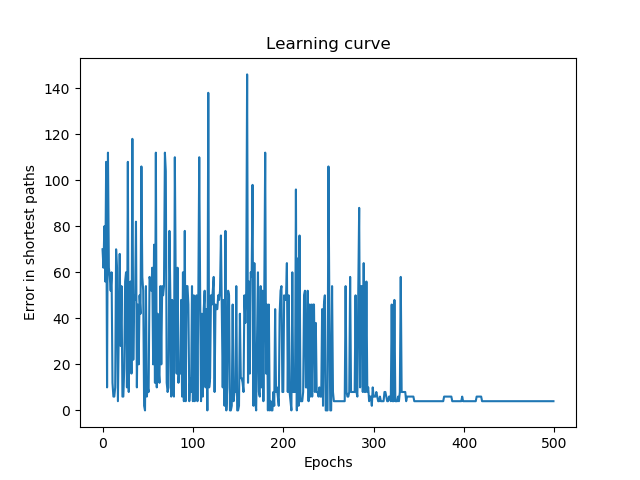
\includegraphics[width=0.7\textwidth]{fig/learning_curve.png}
	\caption{The learning curve of the algorithm based on error$_\pi$.}
	\label{learning}
\end{figure}

\begin{figure}[H]
	\centering
	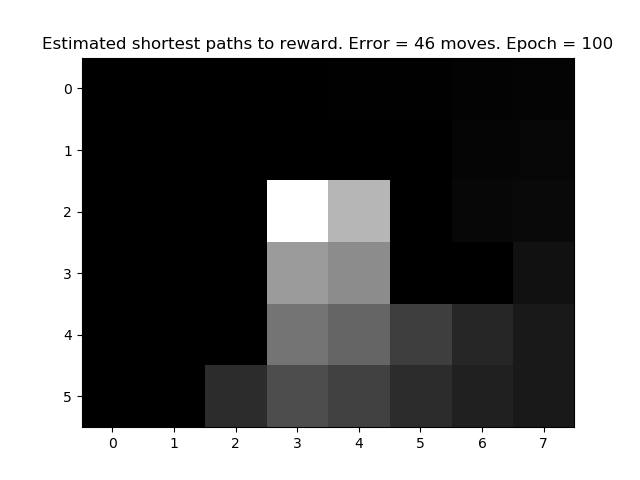
\includegraphics[width=0.31\textwidth]{fig/grid_shortest_paths_100.png}
	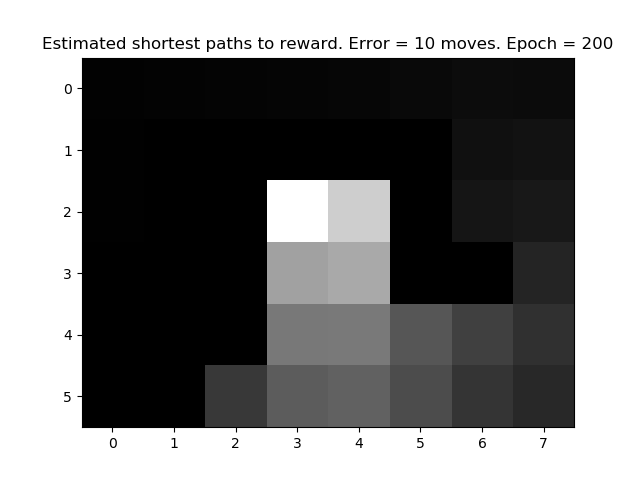
\includegraphics[width=0.31\textwidth]{fig/grid_shortest_paths_200.png}
	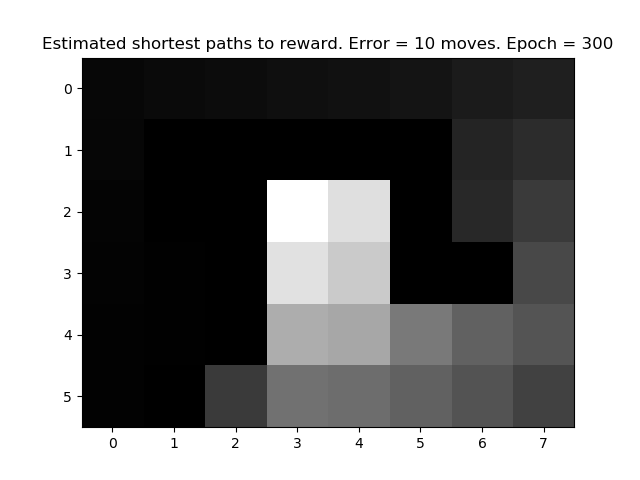
\includegraphics[width=0.31\textwidth]{fig/grid_shortest_paths_300.png}
	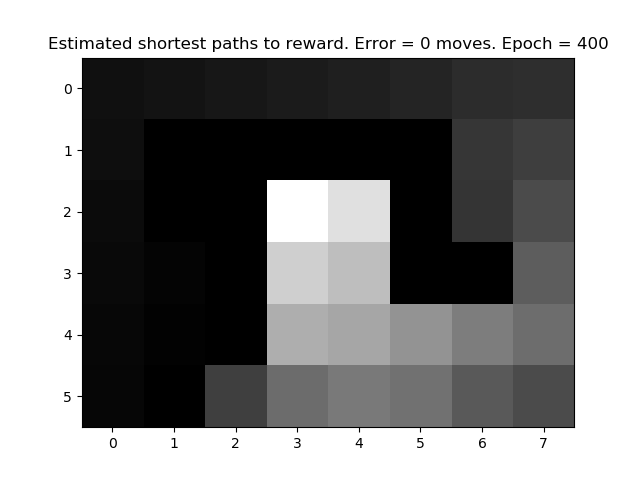
\includegraphics[width=0.31\textwidth]{fig/grid_shortest_paths_400.png}
	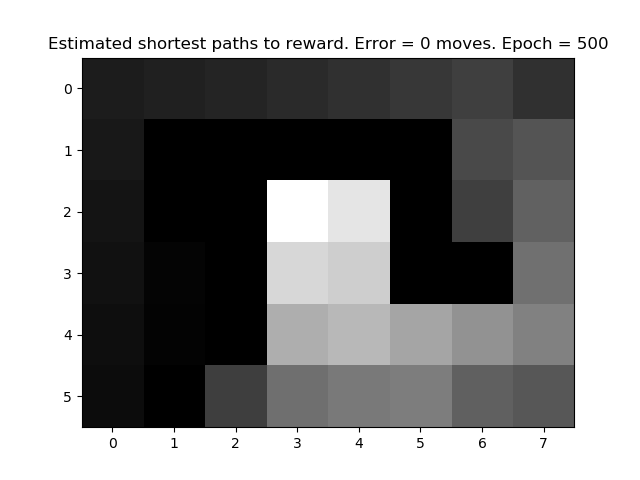
\includegraphics[width=0.31\textwidth]{fig/grid_shortest_paths_500.png}
	\caption{Heatmap of grid after every 100 epochs. This is a visualisation of the shortest paths where the policy is that the agent moves to the brightest adjacent tile.}
	\label{heatmap}
\end{figure}


\begin{figure}[H]
	\centering
	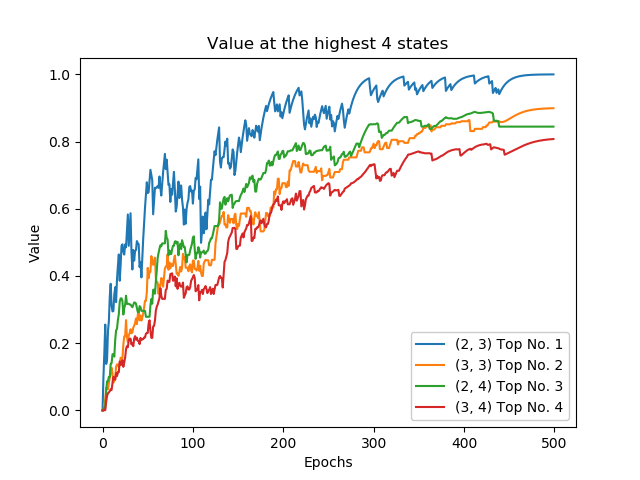
\includegraphics[width=0.7\textwidth]{fig/value_iteration.png}
	\caption{Change in the 4 highest valued states over the epochs.}
	\label{values}
\end{figure}

\section*{Question 2}
The RL algorithm is highly relatable to areas of the brain such as the dopaminergic systems \cite{roelfsema2018control} which code for unexpected reward. Most of the dopamine neurones of the brain originate from the substantia nigra or the ventral tegmental area of the midbrain \cite{delong2000basal}. 

Recent views discuss the significant role of the neurotransmitter dopamine in  goal-directed behavior, cognition, attention, and reward \cite{schultz2002getting}. Specifically in the case of rewards, a study on primates conducted in 1993 \cite{schultz1993responses} and later analysed in 1997 \cite{schultz1997neural} \cite{schultz1998predictive} developed an understanding of the function of the basal ganglia by a series of experiments on the activity of midbrain dopamine. 

The experiments involved providing a monkey with a liquid reward upon learning a new task. During learning, the monkey's dopamine neurones responded to the liquid reward after completing the task. However, upon learning the task, the monkey's neurones respond to the a visual stimulus (a small light) before and cease to respond to the actual stimulus. This showed that the activity of dopamine neurones is affected not only by the present reward, but also the prediction of future rewards. The study also showed that when there was a delay in the reward after the visual stimulus, the dopamine neurones are depressed lower than their basal firing rates. This ties in very well with RL with TD learning. The TD-error $\delta_t$ (reward prediction error) of the TD learning rule behaves exactly like the dopamine neurones of the brain \cite{doya2000complementary}.

An analysis and comparison to the RL model \cite{berns1998computational} \cite{dayan2002reward} showed that the input site of the basal ganglia is made of the striosome and the matrix. The striosome receives signals from the dopamine neurones of the substantia nigra pars conpacta (SNc) and the matrix receives receives output signals from the basal ganglia (substantia nigra pars reticulata and globus palidus). The model elaborates that the striosome is responsible for the reward at the current state whereas the matrix is responsible for future expected rewards.

% It's not clear how the TD error is calculated leading up to the substantia nigra. So we don't know if it is calculated the way we model it in the algorithm \cite{doya2000complementary}.

\section*{Question 3}

RL has a significant biological plausability over supervised learning as RL with TD learning has been shown to mimic the dopamine neurones in the mid-brain \cite{doya2000complementary}. However, backpropagation of action potentials have been shown to not be equivalent to the backpropagation algorithm used in supervised and non-supervised learning \cite{stuart1997action}. 

RL has the ability to know when it is doing well, by virtue of the rewards obtained (or expected rewards). However, unsupervised learning has no way of understanding whether what has been learnt is truely correct. 

Both supervised and unsupervised learning require tremendous amounts or difficult to obtain data before being able to make predictions. Additionally, once given a set of data, the goal is to find a good model of the data given. On the other hand, RL with TD learning learns on-the-go (online learning). It has the capability to explore an environment further (gather more data) to learn better. This mimics animals more closely as they are very rarely limited by a subset of data, and can explore the environment to learn more about it.

\section*{Question 4}

In an environment with a very large state space, the agent would need to acumulate large amounts of data through exploration to make some reasonable policy for navigating the environment. We can overcome this by mapping the set of states as parameterized functions \cite[Chapter 10]{sutton1998introduction} which would require less data to get an approximation of the optimal policy. Realistically, an environment with discrete states doesn't well represent a world with continuous states and so the environment of which an RL agent learns in is fundamentally different from the one animals learn in. 

It has been shown that novel sensory stimuli induce similar activity to that of dopamine cells on unpredicted rewards \cite{kakade2002dopamine}. The difference being that as the stimuli becomes familiar, activity diminishes. This was reasonded as novelty itself having rewarding characteristics \cite{reed1996intrinsic} (intrinsic-motivation \cite{dayan2002reward}). The algorithm we have used doesn't cater for the intrinsically-motivated rewards. Biologically, the intrinsic-motivation encourages exploration which we modelled by the epsilon-greedy mechanism $\epsilon$. However, this isn't motivated by the novelty of a stimuli (or state in our case).

Sutton and Barto identify this shortcomming and note that an animal's reward signals are determined by processes within its brain that monitor both the animal's external and internal state \cite{sutton1998introduction}. Barto et al goes on to develop an \textit{Intrinsically-Motivated RL} model \cite{chentanez2005intrinsically} described in Figure \ref{fig:Internal-External}.

\begin{figure}[H]
	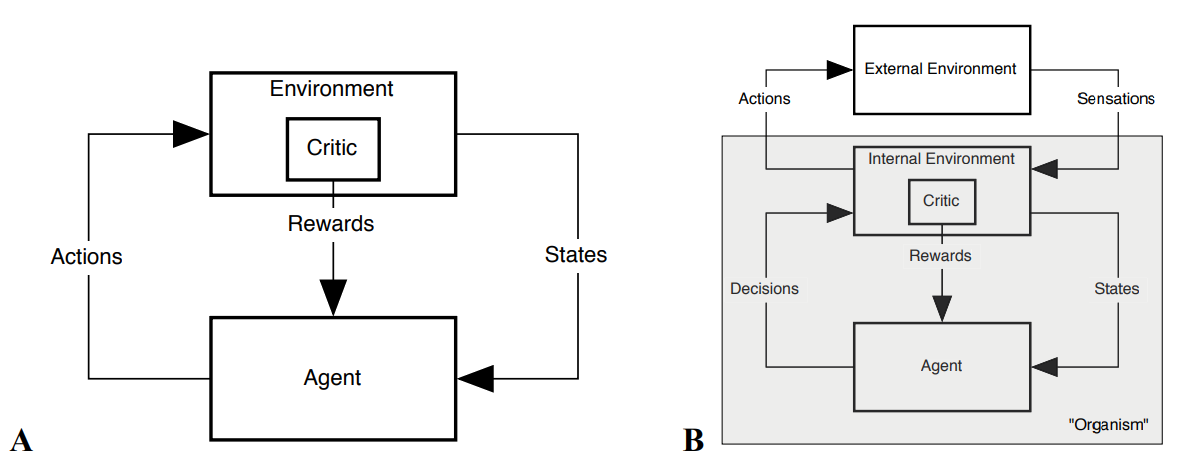
\includegraphics[width=\textwidth]{Q4-Internal-External-Environment.png}
	\caption{Agent-Environment Interaction in RL. \textbf{A}: The usual view. \textbf{B}: An elaboration where the internal environment of the model characterises the organism, in particular, it's motivational system \textit{Sourced from \cite{chentanez2005intrinsically}}.}.
	\label{fig:Internal-External}

\end{figure}

\newpage

\printbibliography

\end{document}
